% examples
% - mnist
% - imdb
% - ARN / ADN 
% - NER (segmentation)
\begin{frame}{Image classification}
  \begin{center}
    \tikz[baseline=0]{ \node at (-2,0)
      {\includegraphics[height=0.25\textheight]{figs/mnist_5.pdf}}; %
      \node at (-0.4,0) {:}; \xvector{0}{-0.75}{6} }
    $\x \in \real^{784} \ \longrightarrow \class  \in\{0, 1,2, \ldots ,9
    \}$
  \end{center}
  \begin{itemize}
  \item $\dataset= (\exi , \classi )_{i=1}^{\nsamples}$ 
  \item \important{Supervised} learning of a \important{classification} task
  \end{itemize}
\end{frame}

\begin{frame}{Review classification}
  \begin{center}
    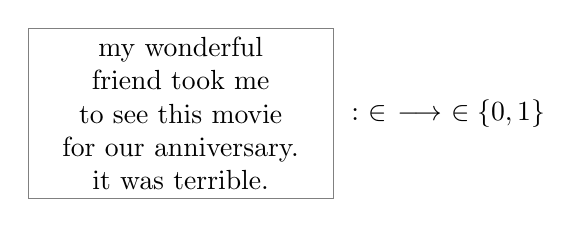
\begin{tikzpicture}
        %%%%%%%%%%%%%%%%%%%%%
      \node[anchor=east,draw=gray,text width=0.3\textwidth,align=center] (review) at
      (0,0) {my wonderful friend took me to see this movie \\for our
        anniversary. \\ it was terrible.};
      %%%%%%%%%%%%%%%%%%%%%
      \node[anchor=west] (txt) at (0.1,0) {$: \ \x \in \real^{\nfeats} \ \longrightarrow \ \class \in\{0, 1\}$};
    \end{tikzpicture}
  \end{center}

  \begin{itemize}
  \item $\dataset= (\exi , \classi )_{i=1}^{\nsamples}$ 
  \item The input is a sequence $\rightarrow$ how to build $\x$ ? 
  \item A sequence of words (discrete symbols)
  \item Words interact with each other, the neighborhood is important
  \end{itemize}
\end{frame}


%%%%%%%%%%%%%%%%%%%%%%%%%%%%%%%%%%%%%%%%%%%%%%%%%%%%%%%%%%%%%%%%%%%%%%%%%%%%%%%%%%%%
% https://en.wikipedia.org/wiki/Enhancer_(genetics)
% https://fr.wikipedia.org/wiki/Amplificateur_(biologie)
%
% In genetics, an enhancer is a short (50–1500 bp) region of DNA that
% can be bound by proteins (activators) t
%
% 3 articles :
% 2 on convNet 
% - https://www.ncbi.nlm.nih.gov/pmc/articles/PMC5773911/
% - https://www.biorxiv.org/content/10.1101/264200v2.full
% 1 on SVM k-mers
% https://www.ncbi.nlm.nih.gov/pubmed/21875935/
%%%%%%%%%%%%%%%%%%%%%%%%%%%%%%%%%%%%%%%%%%%%%%%%%%%%%%%%%%%%%%%%%%%%%%%%%%%%%%%%%%%%
% Alphabet = set of nucleotides: 
% A,C,G,T
\newcommand{\cga}{{\color{red!70!black} A}}
\newcommand{\cgc}{{\color{blue!70!black} C}}
\newcommand{\cgg}{{\color{yellow!70!black} G}}
\newcommand{\cgt}{{\color{green!70!black} T}}
\begin{frame}{Enhancer Identification in  DNA Sequences}
  \framesubtitle{From~\cite{Xu17Enhancer,Cohn18Enhancer}}
  \begin{quote}
    \small Enhancer sequences regulate the expression of genes from
    afar by providing a binding platform for transcription factors,
    (...). Despite
    their importance in health and disease, our understanding of these
    DNA sequences, and their regulatory grammar, is limited. This
    impairs our ability to identify new enhancers along the genome, or
    to understand the effect of enhancer mutations and their role in
    genetic diseases.
  \end{quote}
  \begin{block}{Sequence classification task / property identification}
    \begin{center}
      \begin{tikzpicture}
        %%%%%%%%%%%%%%%%%%%%% 
        \node[anchor=east,draw=gray,text width=0.3\textwidth,align=center] (review) at
        (0,0) {\cga~\cgt~\cgc~\cgg~\cga~\cgt~\cgc~\cgg\\$\cdots$~\cgg~\cgt~\cga~\cga~\cgt~\cgc~\cgg};
        %%%%%%%%%%%%%%%%%%%%% 
        \node[anchor=west] (txt) at (0.1,0) {$: \ \x \in \real^{\nfeats} \ \longrightarrow \ \class \in\{0, 1\}$};
      \end{tikzpicture}
    \end{center}
    \begin{itemize}
    \item Long sequence (arbitrary length)
    \item Only 4 discrete symbols, but  some subsequences are more informative (segments ?)
    \item Long range interactions between segments 
    \end{itemize}
  \end{block}
\end{frame}

\begin{frame}{Predicting the sequence specificities of DNA- and RNA-binding proteins}
  \framesubtitle{from \cite{Alipanahi15DNABinding}}
    \begin{quote}
      \small Knowing the sequence specificities of DNA- and
      RNA-binding proteins is essential for developing models of the
      regulatory processes in biological systems and for identifying
      causal disease variants.
  \end{quote}
  \begin{block}{Sequence classification / regression task}
    \begin{center}
      \begin{tikzpicture}
        %%%%%%%%%%%%%%%%%%%%%
        \node[anchor=east,draw=gray,text width=0.3\textwidth,align=center] (review) at
        (0,0) {\cga~\cgt~\cgc~\cgg~\cga~\cgt~\cgc~\cgg\\$\cdots$~\cgg~\cgt~\cga~\cga~\cgt~\cgc~\cgg};
        %%%%%%%%%%%%%%%%%%%%% 
        \node[anchor=west] (txt) at (0.1,0) {$: \ \x \in \real^{\nfeats} \ \longrightarrow \ \class \in\{0, 1\}\ or\ y \in \real$};
      \end{tikzpicture}
    \end{center}
    \begin{itemize}
    \item The data come in qualitatively different forms:
      \begin{itemize}
      \item Protein binding microarrays (PBMs) and RNAcompete assays
        provide a specificity coefficient for each probe sequence
      \item chromatin mmunoprecipitation (ChIP)-seq10 provides a
        ranked list of putatively bound sequences of varying length;
      \item HT-SELEX11 generates a set of very high affinity
        sequences.
    \end{itemize}
    \item Each  acquisition technology has its own artifacts, biases and limitations
    \end{itemize}
  \end{block}
\end{frame}



\begin{frame}{Audio classification / segmentation}
  \framesubtitle{\cite{Jang19Music}}
  \begin{center}
    \includegraphics[width=0.5\textwidth]{../figs/music_speech}    
  \end{center}
  \begin{itemize}
  \item Classification at each time step
  \item But the context is crucial (for the input and the output) ! 
  \end{itemize}
\end{frame}



\begin{frame}{Sequence generation}
  \begin{block}{Predicting the evolution of a dynamical system}
    \begin{columns}
      \column{0.5\textwidth}
      \begin{center}
        \includegraphics[width=\textwidth]{../figs/ks_h}
      \end{center}
      \column{0.5\textwidth}
      $$P(\y_{1:T}) = \prod_{i=1}^{T} P(\y_i | \y_{1:i-1})$$
    \end{columns}
  \end{block}
  \begin{block}{Sequence generation for sparse observation}
    \begin{columns}
      \column{0.5\textwidth}
      \begin{center}
        \includegraphics[width=\textwidth]{../figs/cylinder}
      \end{center}
      \column{0.5\textwidth}
      $$P(\y_{1:T}| \x ) = \prod_{i=1}^{T} P(\y_i | \y_{1:i-1}, \x)$$
    \end{columns}
  \end{block}
\end{frame}


\begin{frame}{Sequence tagging}
  \begin{align*}
   \wseq = \ws_{1}^{\length} &= \ws_1, \ws_2, ..., \ws_{\length}\\
   \tseq = \tsymb_{1}^{\length} &= \tsymb_1, \tsymb_2, ..., \tsymb_{\length}
  \end{align*}

  Example : Part-of-Speech (POS) tagging\\
  
  \begin{center}
    \begin{tabular}{l|l}
      Sentence &POS-tags\\\hline
      Er &PPER-case=nom$|$@gender=masc$|$number=sg$|$person=3\\
      fürchtet  &VVFIN-mood=ind$|$number=sg$|$person=3$|$tense=pres \\
      noch &ADV \\
      Schlimmeres &NN-case=acc$|$gender=neut$|$number=sg\\
      . &\$. 
    \end{tabular}
  \end{center}
\end{frame}


\newcolumntype{B}{>{\centering\arraybackslash} m{0.3\textwidth}}  %# New column type
\newcolumntype{C}{>{\centering\arraybackslash} m{0.25\textwidth}}  %# New column type
\begin{frame}{Speech recognition / Machine Translation}
    \begin{center}
    \begin{tabular}{B|C}
      \textit{Input} & \textit{Output}\\\hline
      \includegraphics[width=0.3\textwidth]{../figs/Signal-speech-martin-de.png} & $[$ Martine, boude $]$\\\hline\pause
      \multirow{3}{*}{$[$ il, est, temps $]$} & \multirow{3}{*}{$[$ es , ist , zeit $]$}   \\
      & \\
      &\\\hline\pause
      \multirow{3}{*}{$ \mathbf{x}  $} & \multirow{3}{*}{$\mathbf{y} = (y_1,  y_2, ... , y_I)$}  \\ & \\ & \\\hline
    \end{tabular}
  \end{center}\pause
    \begin{block}{\centering$P( \mathbf{y} | \mathbf{x}) = \prod_i^I P( y_i |\mathbf{y_{<i}},\mathbf{x}) $}
      \begin{itemize}
      \item Generate $\mathbf{y} $ from $\mathbf{x}$
      \item Evaluate $\mathbf{y}$ in the context $\mathbf{x}$
      \end{itemize}
    \end{block}
  % \begin{columns}
  %   \column{0.1\textwidth} 
  %   $$
  %   P( \mathbf{y} |  \mathbf{x}) \rightarrow
  %   $$
  %   \column{0.5\textwidth}
  %   \begin{itemize}
  %   \item Evaluate $\mathbf{y}$ in the context $\mathbf{x}$
  %   \item Generate $\mathbf{y} $ from $\mathbf{x}$
  %   \end{itemize}
  % \end{columns}
\end{frame}

\begin{frame}{Sequence in machine learning}
  \begin{block}{Sequence classification / regression}
    \begin{itemize}
    \item A sequence as input (of arbitrary length)
    \item Made of discrete symbols of real vectors 
    \item[$\rightarrow$] Predict a value, a class as output 
    \item[$\rightarrow$] Extract features from the sequence (summarize/compress)
    \item[$\rightarrow$] Represent the sequence as a whole to make a prediction
    \end{itemize}
  \end{block}
  \begin{block}{Generative sequence model}
    $$P( \mathbf{y} | \mathbf{x}) = \prod_i^I P( y_i |\mathbf{y_{<i}},\mathbf{x}) $$
  \end{block}
\end{frame}

\begin{frame}{Unsupervised pre-training and supervised fine-tuning}
  \begin{quote}
    Anotated datasets are usually scarce and sparse, while unannotated
    data are readily available
  \end{quote}
  \begin{block}{Unsupervised pre-training}
    Train a generative model of the input sequence: 
    $$P_{\params}( x_i |\mathbf{x_{<i}}) $$
    on unannotated data
  \end{block}
  \begin{block}{Supervised fine-tuning}
    Train a classifier $P_{\boldsymbol{\phi}} (\classi | \exi)$ on annotated dataset, but:
    \begin{itemize}
    \item Initialize some parameters (part of $\boldsymbol{\phi}$) with some parts of $\params$
    \item Optionally fine tune them. 
    \end{itemize}
  \end{block}

  
\end{frame}

\begin{frame}{DNA Sequence \textit{vs} Sentence classification}
  \begin{block}{Text representation}
    \begin{itemize}
    \item a text is a structured sequence made of words;
    \item a word is a discrete symbol;
    \item belonging to a \textit{finite} set: the vocabulary $\vocab$. 
    \end{itemize}
  \end{block}
  \begin{block}{Compositionality}
    \begin{itemize}
    \item {The meaning of a complex expression is determined by the
        meanings of its constituent,}
    \item {\color{red}and the rules used to combine them. }
    \end{itemize}
  \end{block}
  \begin{block}{DNA sequence}
    \begin{itemize}
    \item Potentially very long sequence made of 4 discrete symbols
    \item Subsequences can be compared to words, but the segmentation is missing
    \item Complexe interaction with long range dependancies 
    \end{itemize}
  \end{block}
\end{frame}

\endinput


